\documentclass[11pt]{article}

\usepackage[a4paper,margin=2.5cm]{geometry}
\usepackage{parskip}
\usepackage{xcolor}
\usepackage{listings}
\usepackage{hyperref}
\usepackage{enumitem}
\usepackage{booktabs}
\usepackage{tikz}
\usetikzlibrary{positioning,arrows.meta}
\usepackage{fancyhdr}
\usepackage{titlesec}
\usepackage{graphicx}

\definecolor{codebg}{RGB}{245,245,245}
\definecolor{codekw}{RGB}{0,90,150}

\lstdefinestyle{sh}{
  backgroundcolor=\color{codebg},
  basicstyle=\ttfamily\small,
  frame=single,
  rulecolor=\color{gray!40},
  breaklines=true,
  columns=fullflexible,
  keywordstyle=\color{codekw}\bfseries,
  showstringspaces=false,
}
\lstset{style=sh}

\lstdefinestyle{clisting}{
  backgroundcolor=\color{codebg},
  basicstyle=\ttfamily\scriptsize,
  frame=single,
  rulecolor=\color{gray!40},
  breaklines=true,
  columns=fullflexible,
  keywordstyle=\color{codekw}\bfseries,
  commentstyle=\color{gray!60}\itshape,
  showstringspaces=false,
  language=C,
  tabsize=4,
}

\titleformat{\section}{\Large\bfseries}{\thesection}{0.6em}{}
\titleformat{\subsection}{\large\bfseries}{\thesubsection}{0.6em}{}

\pagestyle{fancy}
\fancyhf{}
\fancyhead[L]{
\includegraphics[height=0.75cm]{edge.png}}
\fancyhead[C]{\small\textsc{X-HEEP Accelerator Labs} --- Lab 0}
\fancyhead[R]{
\includegraphics[height=0.75cm]{polito.png}}
\fancyfoot[C]{\thepage}
\renewcommand{\headrulewidth}{0.4pt}

\newcommand{\code}[1]{\texttt{#1}}

\begin{document}

% ---------------------------------------------------------------- Title page
\begin{titlepage}
\thispagestyle{empty}
\centering
\vspace*{1.5cm}


\includegraphics[height=3.6cm]{polito.png}

\vspace{1.2cm}


\includegraphics[height=4.2cm]{edge.png}

\vspace{2.2cm}

{\Huge\bfseries Lab 0: Profiling \& Accelerator Proposal\par}

\vspace{0.8cm}

{\Large X-HEEP Accelerator Labs\par}

\vspace{0.4cm}

{\large A custom hardware accelerator design lab\par}

\vfill

{\large Politecnico di Torino \par}

\vspace{0.3cm}

{\large EDGE Group\par}

\vspace{1cm}

\end{titlepage}

% ------------------------------------------------------------- Content pages
\pagestyle{fancy}

\section*{Objective}

Select one of the four applications below, profile it on X-HEEP, and decide
which piece of it you would build custom hardware for. That is the whole
lab: no RTL yet, just evidence. The four applications are not toy loops
invented for the occasion --- each one is a small, integer-only
implementation of a kernel that shows up, in a much bigger form, inside a
real system described in a real paper. Two of them (\code{matmul},
\code{crc32}) are single, homogeneous kernels: profiling tells you ``how
expensive is this loop''. The other two (\code{tinyconv}, \code{attention})
are small \emph{pipelines} of two or three sub-kernels, closer to what a real
accelerator design problem looks like: profiling has to tell you \emph{which
of several candidate pieces} is worth accelerating, and the honest answer is
not always the one that looks the most obviously ``hardware-shaped'' on
paper.

\section{The applications}

All four live under \code{sw/applications/<name>/main.c}, already wired with
the \code{PROFILE\_START}/\code{PROFILE\_END} macros from
\code{sw/external/profile.h} around the region(s) you should profile. Read
the code before you run it --- you are going to have to explain, in the
proposal, exactly what is happening inside the loop you propose to
accelerate.

\subsection{matmul --- integer matrix multiply}

A $16\times16$ integer GEMM (general matrix multiply): the single triple-nested
loop below. GEMM is the arithmetic core of essentially every neural-network
layer once weights and activations are quantized to low-precision integers
for embedded inference \cite{jacob2018quantization} --- both applications
further down this list reduce to GEMM internally. It is also the canonical
first accelerator target: regular access pattern, full data reuse, an
obvious mapping to a MAC array or systolic array.

\begin{lstlisting}[style=clisting]
#define N 16
static int32_t a[N][N], b[N][N], c[N][N];

static void matmul(void) {
    for (int i = 0; i < N; i++)
        for (int j = 0; j < N; j++) {
            int32_t acc = 0;
            for (int k = 0; k < N; k++)
                acc += a[i][k] * b[k][j];
            c[i][j] = acc;
        }
}
\end{lstlisting}

\subsection{crc32 --- CRC-32 checksum}

A bit-serial CRC-32 (the IEEE 802.3 polynomial) over a 256-byte buffer, the
classic error-detecting code used in Ethernet frames and countless storage
and communication protocols \cite{peterson1961cyclic}. Unlike \code{matmul},
this kernel is control-heavy and touches one bit at a time: a poor fit for a
wide MAC array, but a very good fit for a small, tightly-coupled instruction
extension, or a tiny bit-serial state machine behind a memory-mapped
register.

\begin{lstlisting}[style=clisting]
static uint32_t crc32(const uint8_t *data, int len) {
    uint32_t crc = 0xFFFFFFFFu;
    for (int i = 0; i < len; i++) {
        crc ^= data[i];
        for (int b = 0; b < 8; b++) {
            uint32_t mask = -(crc & 1u);
            crc = (crc >> 1) ^ (0xEDB88320u & mask);
        }
    }
    return ~crc;
}
\end{lstlisting}

\subsection{tinyconv --- a CNN convolution layer}

A single Conv2D + ReLU layer: a $3{\times}3$ kernel, 2 input channels, 4
output channels, int8 activations/weights with int32 accumulation, over a
$10{\times}10$ input. This is the same layer structure as the convolutional
layers in LeNet-5 \cite{lecun1998gradient}, the architecture that established
the conv+ReLU+pool pattern used by essentially every CNN since, executed here
the way an embedded accelerator actually would: as pure integer arithmetic,
in the style of integer-only quantized inference \cite{jacob2018quantization}
rather than floating point.

The kernel is six nested loops instead of three: the outer four walk output
channels and output pixels, the inner two slide a $3{\times}3$ window over
the input. It is still ``just'' a lot of MACs, but with a \emph{sliding
window} access pattern instead of full reuse --- the interesting hardware
question is how much of that window you can keep resident instead of
re-reading it from memory for every output pixel.

\begin{lstlisting}[style=clisting]
#define CIN  2
#define COUT 4
#define K    3
#define IH   10
#define IW   10
#define OH  (IH - K + 1)
#define OW  (IW - K + 1)

static int8_t  in[CIN][IH][IW];
static int8_t  weight[COUT][CIN][K][K];
static int32_t bias[COUT];
static int32_t out[COUT][OH][OW];

static void conv2d_relu(void) {
    for (int f = 0; f < COUT; f++)
        for (int oy = 0; oy < OH; oy++)
            for (int ox = 0; ox < OW; ox++) {
                int32_t acc = bias[f];
                for (int c = 0; c < CIN; c++)
                    for (int kh = 0; kh < K; kh++)
                        for (int kw = 0; kw < K; kw++)
                            acc += (int32_t)in[c][oy + kh][ox + kw] *
                                   (int32_t)weight[f][c][kh][kw];
                out[f][oy][ox] = acc > 0 ? acc : 0;  // ReLU
            }
}
\end{lstlisting}

\subsection{attention --- single-head scaled dot-product attention}

A single attention head, the mechanism at the heart of the Transformer
\cite{vaswani2017attention}, run over a short sequence ($8$ tokens, model
dimension $8$) in fixed-point integer arithmetic. Unlike the other three
applications, this one is deliberately split into \textbf{three} separately
profiled sub-kernels, because that is the actual design question a
Transformer accelerator faces:

\begin{enumerate}[nosep]
  \item \code{qk\_matmul} --- $\mathrm{scores} = Q \cdot K^\top$ (a GEMM,
        exactly like \code{matmul/}).
  \item \code{softmax} --- row-wise normalization of the scores into
        attention weights.
  \item \code{av\_matmul} --- $\mathrm{out} = \mathrm{weights} \cdot V$
        (a GEMM again).
\end{enumerate}

A real softmax needs an exponential and a division, neither of which is
pleasant in integer-only hardware. The implementation below uses a
shift-based approximate exponential --- decay by a power of two instead of
$e^x$ --- in the spirit of hardware-oriented softmax designs such as
Softermax \cite{stevens2021softermax} and integer-only Transformer inference
such as I-BERT \cite{kim2021ibert}; it is simplified for teaching and is
\emph{not} a faithful reproduction of either paper. The final per-row
normalization still uses one integer division per element, which is exactly
the kind of detail profiling is for: does that division-heavy loop actually
dominate, or do the two matmuls?

\begin{lstlisting}[style=clisting]
#define SEQ 8
#define DM  8
#define WEIGHT_ONE  256   // fixed-point "1.0", Q8
#define DECAY_SHIFT 2

static int8_t  Q[SEQ][DM], K[SEQ][DM], V[SEQ][DM];
static int32_t scores[SEQ][SEQ], weights[SEQ][SEQ], out[SEQ][DM];

// 1. scores[i][j] = Q[i] . K[j]
static void qk_matmul(void) {
    for (int i = 0; i < SEQ; i++)
        for (int j = 0; j < SEQ; j++) {
            int32_t acc = 0;
            for (int d = 0; d < DM; d++)
                acc += (int32_t)Q[i][d] * (int32_t)K[j][d];
            scores[i][j] = acc;
        }
}

// 2. row-wise softmax, shift-based integer exponential approximation
static void softmax(void) {
    for (int i = 0; i < SEQ; i++) {
        int32_t row_max = scores[i][0];
        for (int j = 1; j < SEQ; j++)
            if (scores[i][j] > row_max) row_max = scores[i][j];

        int32_t sum = 0;
        for (int j = 0; j < SEQ; j++) {
            int32_t diff = row_max - scores[i][j];       // >= 0
            int32_t shift_amt = diff >> DECAY_SHIFT;
            int32_t w = (shift_amt < 31) ? (WEIGHT_ONE >> shift_amt) : 0;
            weights[i][j] = w;
            sum += w;
        }
        if (sum == 0) sum = 1;
        for (int j = 0; j < SEQ; j++)
            weights[i][j] = (weights[i][j] * WEIGHT_ONE) / sum;  // divide
    }
}

// 3. out[i] = sum_j weights[i][j] * V[j]
static void av_matmul(void) {
    for (int i = 0; i < SEQ; i++)
        for (int d = 0; d < DM; d++) {
            int32_t acc = 0;
            for (int j = 0; j < SEQ; j++)
                acc += weights[i][j] * (int32_t)V[j][d];
            out[i][d] = acc / WEIGHT_ONE;
        }
}
\end{lstlisting}

\section{Commands}

Set up once, then build and run each application in turn. Each run prints one
profiling line per \code{PROFILE\_START}/\code{PROFILE\_END} pair --- one line
for \code{matmul} and \code{crc32}, three lines for \code{attention}.

\begin{lstlisting}[language=bash]
make vendor                            # pull X-HEEP into ./x-heep
make mcu-gen                           # generate the MCU from config.py
make verilator-build                   # build the Verilator model

make app PROJECT=matmul                # compile matmul
make verilator-run PROJECT=matmul      # run it (prints cycle/instr count)

make app PROJECT=crc32                 # compile crc32
make verilator-run PROJECT=crc32       # run it (prints cycle/instr count)

make app PROJECT=tinyconv              # compile tinyconv
make verilator-run PROJECT=tinyconv    # run it (prints cycle/instr count)

make app PROJECT=attention             # compile attention
make verilator-run PROJECT=attention   # run it (prints 3 cycle/instr lines)

make profile                           # flamegraph from the last run's .fst
make verilator-waves                    # inspect waveforms (gtkwave)
\end{lstlisting}

\section{Reading the output: an example}

Profiling gives you three different views of the same run. Here is what each
one actually looks like, and how to read it.

\subsection{Cycle-count \code{printf} output}

This is what \code{make verilator-run} prints, straight from the
\code{PROFILE\_START}/\code{PROFILE\_END} macros. Here it is for
\code{matmul} and \code{crc32} on the reference build:

\begin{lstlisting}[language=bash]
$ make app PROJECT=matmul && make verilator-run PROJECT=matmul
[profile] matmul: 68199 cycles, 30580 instr
matmul 16x16 checksum=0x...

$ make app PROJECT=crc32 && make verilator-run PROJECT=crc32
[profile] crc32: 20227 cycles, 15621 instr
crc32 len=256 result=0x...
\end{lstlisting}

\textbf{How to read it:} \code{cycles} is how long the bracketed region took
on the simulated core; \code{instr} is how many instructions it dynamically
executed to get there. Two things follow directly from these two numbers:

\begin{itemize}[nosep]
  \item \textbf{Absolute cost.} \code{matmul} costs about $3.4\times$ more
        cycles than \code{crc32} for its kernel --- on its own this only
        tells you which region is more expensive, not why.
  \item \textbf{Cycles per instruction (CPI).} Divide the two: \code{matmul}
        is $68199/30580 \approx 2.2$ cycles/instr, \code{crc32} is
        $20227/15621 \approx 1.3$ cycles/instr. A CPI close to 1 means the
        core is mostly retiring one instruction per cycle (compute-bound,
        few stalls); a higher CPI hints at stalls --- waiting on memory,
        mispredicted branches, or multi-cycle operations (a division, for
        instance). This is often the first clue about \emph{why} a kernel is
        slow, before you even open a flamegraph.
\end{itemize}

For \code{attention}, the same run instead prints \emph{three} lines, one per
sub-kernel, in this format (illustrative values --- run it yourself to get
real ones):

\begin{lstlisting}[language=bash]
[profile] qk_matmul: <cycles> cycles, <instr> instr
[profile] softmax:   <cycles> cycles, <instr> instr
[profile] av_matmul: <cycles> cycles, <instr> instr
attention seq=8 dm=8 checksum=0x...
\end{lstlisting}

This is the point of splitting the profiling: with one number, there is
nothing to decide. With three, you do --- and the answer is not obvious from
reading the code alone. The two matmuls (\code{qk\_matmul}, \code{av\_matmul})
look like the ``hardware-shaped'' part; but \code{softmax} does an integer
\emph{division} per element, and division is expensive on a small RISC-V
core. Whether the matmuls or the division-heavy normalization actually
dominate is exactly the kind of question you cannot answer by inspection ---
it is why this lab makes you measure before you design anything. Compare the
CPI of the three sub-kernels the same way as above: a \code{softmax} CPI
noticeably higher than the two matmuls' is the profiler telling you, in one
number, that the division loop is stalling the core far more per instruction
than the MACs are.

\subsection{\code{RV\_PROFILE} flamegraph output}

\code{make profile} turns the waveform from your last run into a flamegraph
(\code{x-heep/util/profile/flamegraph.svg}), an \emph{icicle plot} of which
functions were on the call stack, and for how long. Figure~\ref{fig:flame}
sketches what one looks like for \code{matmul} (illustrative proportions, not
measured pixel-for-pixel --- open the real SVG to get the real one).

\begin{figure}[h]
\centering
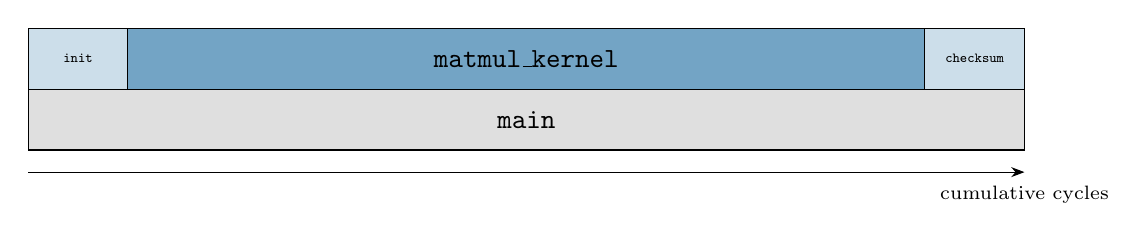
\begin{tikzpicture}[x=1pt,y=1pt]
  % level 0: main, full width
  \draw[fill=gray!25] (0,0) rectangle (360,22);
  \node at (180,11) {\ttfamily main};

  % level 1: init (small) + matmul_kernel (dominant) + checksum (small)
  \draw[fill=codekw!20] (0,22) rectangle (36,44);
  \node[font=\tiny] at (18,33) {\ttfamily init};

  \draw[fill=codekw!55] (36,22) rectangle (324,44);
  \node at (180,33) {\ttfamily matmul\_kernel};

  \draw[fill=codekw!20] (324,22) rectangle (360,44);
  \node[font=\tiny] at (342,33) {\ttfamily checksum};

  % axis
  \draw[-Stealth] (0,-8) -- (360,-8);
  \node[font=\scriptsize] at (360,-16) {cumulative cycles};
\end{tikzpicture}
\caption{How to read a flamegraph: each row is one level of the call stack
(\code{main} at the bottom, callees stacked above it); the \emph{width} of a
box is proportional to the cycles spent in that function (including
whatever it calls); \emph{siblings} are ordered left-to-right, not by time of
call. The widest box --- here \code{matmul\_kernel} --- is where to look
first.}
\label{fig:flame}
\end{figure}

\textbf{How to read it:} width, not position, is the signal. A wide box
means many cycles were attributed to that function; a narrow one means few.
Stacking (a box directly above another) means the top function was called
from the bottom one. If the box for the function you already suspected from
the cycle count (Section~3.1) is indeed the widest one at its level, the two
methods agree and you have a confirmed hotspot; if the widest box is a
function you did \emph{not} expect, that is the flamegraph earning its keep.

\subsection{Waveform inspection}

\code{make verilator-waves} opens the same run's signals in GTKWave. This is
a \textbf{debugging aid only} here, not a numeric measurement: use it to
sanity-check that the bus/memory activity you see during the region actually
lines up with the loop you profiled (e.g., a burst of memory reads exactly
while \code{matmul\_kernel} is running), not to extract a new number.

\section*{What to do with the numbers}

For whichever application you pick, you should be able to point at the
profiling output and say, concretely: this function (or this one sub-kernel
out of several) is where the cycles go, and here is why its shape makes it a
good --- or bad --- candidate for a hardware accelerator.

\begin{thebibliography}{9}
\small

\bibitem{jacob2018quantization}
B. Jacob, S. Kligys, B. Chen, M. Zhu, M. Tang, A. Howard, H. Adam, and D.
Kalenichenko. \emph{Quantization and Training of Neural Networks for
Efficient Integer-Arithmetic-Only Inference}. CVPR, 2018.

\bibitem{lecun1998gradient}
Y. LeCun, L. Bottou, Y. Bengio, and P. Haffner. \emph{Gradient-Based Learning
Applied to Document Recognition}. Proceedings of the IEEE, 86(11), 1998.

\bibitem{vaswani2017attention}
A. Vaswani, N. Shazeer, N. Parmar, J. Uszkoreit, L. Jones, A. N. Gomez, L.
Kaiser, and I. Polosukhin. \emph{Attention Is All You Need}. NeurIPS, 2017.

\bibitem{stevens2021softermax}
J. R. Stevens, R. Venkatesan, S. Dai, B. Khailany, and A. Raghunathan.
\emph{Softermax: Hardware/Software Co-Design of an Efficient Softmax for
Transformers}. DAC, 2021.

\bibitem{kim2021ibert}
S. Kim, A. Gholami, Z. Yao, M. W. Mahoney, and K. Keutzer. \emph{I-BERT:
Integer-only BERT Quantization}. ICML, 2021.

\bibitem{peterson1961cyclic}
W. W. Peterson and D. T. Brown. \emph{Cyclic Codes for Error Detection}.
Proceedings of the IRE, 49(1), 1961.

\end{thebibliography}

\end{document}
